\chapter{Ischemic Heart Disease}
\label{ihd-background}

Ischemic heart disease is a term covering a variety of conditions, 
all caused by myocardial ischemia---%
an imbalance between the coronary blood supply and the 
oxygen requirements of the myocardium.
In the overwhelming majority of cases, 
this imbalance can be attributed to obstructive atherosclerotic disease 
that limits coronary blood flow
~\autocite{kumarRobbins2014}.
In these cases, ischemic heart disease is therefore synonymous 
with coronary artery disease.

The central etiological entity in ischemic heart disease
is therefore the atherosclerotic plaque, 
which is part of the process known as atherosclerosis. 
~\autocite{kumarRobbins2014}
An atherosclerotic plaque consists of blood cells, lipids, calcium 
and connective tissue that are gradually deposited in the arterial wall 
over a number of years.
~\autocite{libbyPathophysiology2005}
The plaque can grow large enough to severely narrow the arterial lumen,
or it can become unstable and as a consequence rupture or erode,
leading to thrombosis.%
\sidenote[][27em]{%
    \fullcite{fusterPathogenesis1992}
}
Both of these scenarios can severely affect 
the perfusion of tissues and organs, 
and when coronary arteries are affected,
it can lead to ischemic heart disease.


\begin{figurefw}
    \centering
    \vspace{-5em}
	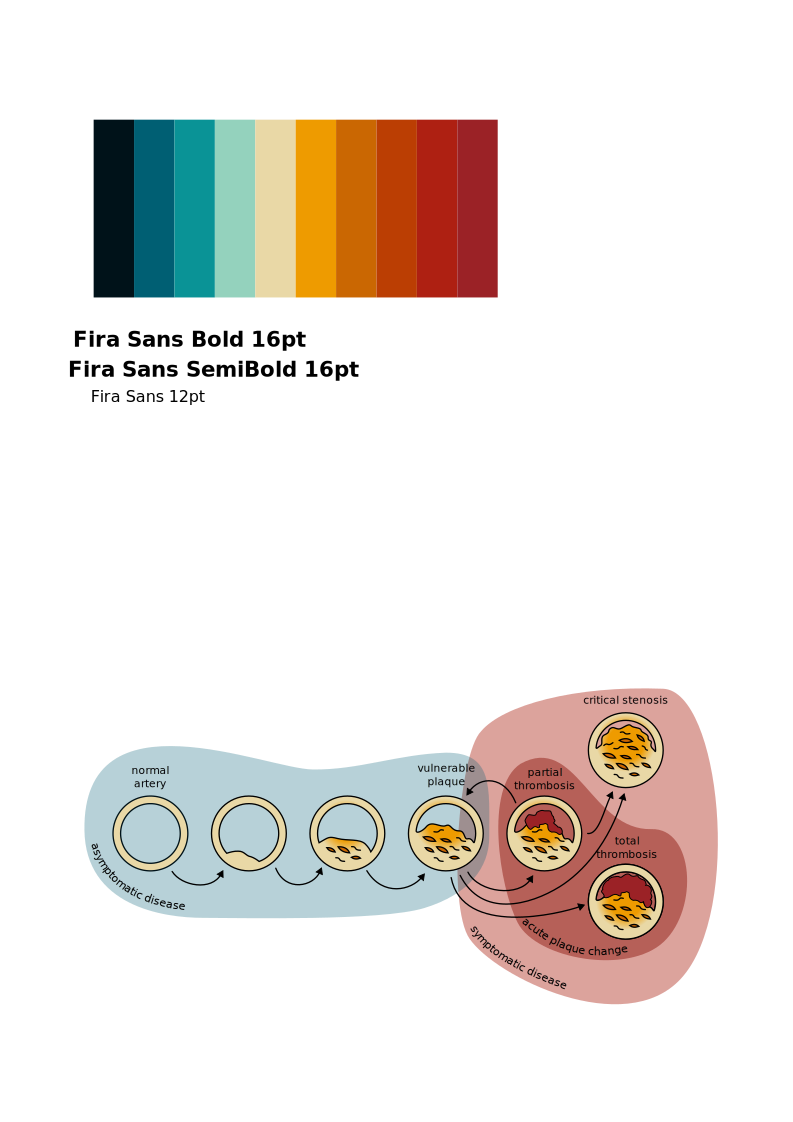
\includegraphics[width=\linewidth]{graphics/atherosclerosis}
    \caption[The process of atherosclerosis]{%
        The atherosclerotic process. 
        From a otherwise normal artery, 
        disruption of endothelial integrity and function, 
        through a combination of genetics and risk factors,
        leads to endothelial injury and low-grade inflammation. 
        Over time, this results in plaque formation through 
        accumulation of lipids, lipoproteins, calcium, and connective tissue.
        Eventually, the plaque may become \enquote{vulnerable}, 
        making it susceptible to sudden rupture or erosion. 
        Such an event can trigger thrombosis and acute changes in the plaque, 
        which, depending on their severity, may either immediately obstruct 
        the arterial lumen%
        ---leading to myocardial infarction or sudden cardiac death---%
        or contribute to further calcification through remodeling. 
        When the progressive narrowing of the arteries reaches a point where 
        it causes symptoms, the stenosis is considered critical, and the 
        myocardium experiences inadequate perfusion, manifesting as angina 
        pectoris.
    }
    \vspace{-5.1em}
    \label{fig:atherosclerosis}
\end{figurefw}

\vspace{9em}

\section{Disease Manifestation}

The pathological process underlying ischemic heart disease 
is inherently chronic with atherosclerotic lesions 
gradually developing over time, 
but in the event of plaque rupture it can abruptly transition
and manifest as an acute condition.
The clinical presentation of ischemic heart disease  
is consequentially diverse and includes both acute 
~\autocite{byrne20232023}
and chronic coronary syndromes.
~\autocite{knuuti20192020}

Acute coronary syndromes includes 
\ac{UA}, \ac{STEMI}, and \ac{NSTEMI},
that collectively represents a spectrum of acute onset or progression of 
myocardial ischemia.
If the ischemia is sufficient to cause myocardial necrosis, 
it is per definition called \ac{MI}~\autocite{thygesenFourth2019}.
\ac{STEMI} and \ac{NSTEMI} are both forms of \ac{MI} that are distinguised
by a characteristic presence or absence of ST-segment elevation on a \ac{ECG}.
All of the acute coronary syndromes are typically associated 
with acute plaque change and atherothrombosis, 
and are medical emergencies that require immediate 
intervention to limit or prevent myocardial damage.
~\autocite{kumarRobbins2014}

\begin{marginfigure}%
    \vspace{1em}
    
\includegraphics{graphics/electrocardiogram}
    \caption[Normal QRS complex]{%
        Schematic of a normal sinus rhythm as seen from an ECG. 
        In \ac{STEMI}, the ST-segment is found elevated.
    }
    \vspace{1em}
    \label{fig:ecg}
\end{marginfigure}%

Chronic coronary syndromes are more stable manifestations of the disease,
and include stable angina and chronic ischemic heart disease.
Stable angina, or \textit{angina pectoris}, is characterised by episodes of
crushing chest pain caused by myocardial ischemia.
By definition, the level of ischemia is not severe enough to lead to
tissue necrosis. 
~\autocite{knuuti20192020}
Unlike \ac{UA}, the symptoms of stable angina are predictable,
are reliably triggered by a specific level of physical exertion, 
and are absent when the individual is at rest. 
Chronic ischemic heart disease can either be a long-term progression of stable
ischemic heart disease or a late-stage stabilization following a \ac{MI} that
has undergone revascularization. 
~\autocite{knuuti20192020}
This condition represents the cumulative
effects of prolonged myocardial ischemia and accrued myocardial damage,
ultimately leading to progressive congestive heart failure.
~\autocite{kumarRobbins2014}

\section{Diagnosis and Treatment}

Since the 1950s, a series of groundbreaking scientific advances have improved 
our understanding and management of cardiovascular disease, leading to a 
drastic decline of mortality in ischemic heart disease.
~\autocite{nabelTale2012}
These advances span from from diagnostic imaging techniques to pharmacological
therapies and surgical interventions, each contributing to a more nuanced
understanding of the disease and more effective treatment options.
~\autocite{nabelTale2012}
To translate this constantly evolving body of knowledge into actionable medical
practice, the European Society of Cardiology (ESC) annually releases
comprehensive clinical practice guidelines that cover a wide array of
cardiovascular conditions.

In line with ESC guidelines, 
invasive management is the recommended approach
for immediate treatment of acute coronary syndromes.
This includes primary \ac{PCI}%
%%%%%%%%%%%%%%%%%%%%%%%%%%%%%%%%%%%%%%%%%%%%%%%%%%%%%%%%%%%%%%%%%%%%%%%%%%%%%%%
\sidenote[][-3em]{%
    \ac{PCI} is a minimally invasive procedure used for treatment of
    atherosclerosis. It involves the use of a small balloon catheter 
    to widen flow-limiting stenoses and restore cardiac perfusion.
} 
%%%%%%%%%%%%%%%%%%%%%%%%%%%%%%%%%%%%%%%%%%%%%%%%%%%%%%%%%%%%%%%%%%%%%%%%%%%%%%%
for \ac{STEMI} and emergency angiography, 
potentially with concurrent \ac{PCI},
for patients with very high-risk \ac{NSTEMI} and \ac{UA}.
For those with a more stable presentation, but still at high-risk, 
angiography within the first 24 hours is indicated to
assess the need for revascularization. 
~\autocite{byrne20232023}
Based on factors such as the coronary anatomy, 
number and grade of stenotic vessels, 
and the estimated risk of surgical complications
\ac{CABG} is sometimes preferred over \ac{PCI}.
~\autocite{neumann20182019}
The primary objective of these interventions 
is providing timely revascularization where needed,
to restore coronary perfusion and limit myocardial damage.

Concurrent with invasive treatment, 
the guideline gives a class I recommendation for initiation 
of antithrombotic therapy. 
~\autocite{byrne20232023}
While the specifics of this therapy is beyond the scope of this thesis,
it generally involves a combination of antiplatelet and anticoagulant 
medications, aimed at preventing further thrombotic events.
~\autocite{nabelTale2012}

Contrastingly, for chronic coronary syndromes,
invasive coronary angiography is typically not 
the first-line diagnostic test.
~\autocite{knuuti20192020}
However, for patients with a high clinical likelihood of ischemic heart
disease, who present with easily induceable or refractory angina pectoris 
and a high event risk, coronary angiography is recommended for assessment of
revascularization options.  
~\autocite{knuuti20192020}

\section{Secondary Prevention}

Once the acute phase of the disease has been stabilized 
through revascularization or other treatments,
the clinical focus shifts to long-term management and secondary prevention.
Patients with established ischemic heart disease are generally of 
high risk of subsequent events, 
particularly if risk factors are not adequately managed.
~\autocite{clarkMetaAnalysis2005}
Guidelines advocate for a multifaceted approach to secondary prevention, 
incorporating lifestyle changes like quitting smoking and starting exercise, 
as well as pharmacological interventions such as lipid-lowering therapies. 
~\autocite{visseren20212021}

The goal of long-term treatment is essentially twofold:
to limit the progression of existing atherosclerotic plaque and 
to prevent and limit thrombus formation if plaques should rupture or erode.
~\autocite{foxMyth2020}
The clinical trajectories of patients with chronic manisfestations of 
ischemic heart disease can remain stable for several years,
before unexpectedly deterioating to 
major adverse cardiovascular events.
~\autocite{foxMyth2020}
For this reason, continuous monitoring and risk factor evaluation 
are recommended to guide secondary prevention therapy.

To tailor treatment plans, risk stratification models that integrate 
clinical characteristics and risk factor profiles can be useful.
~\autocite{visseren20212021}
Such models could potentially help identify patients who are more likely to 
benefit from aggressive therapy. 
However, the implementation and effectiveness of using such risk scores to 
dynamically adjust treatment over time remains an area of active research.
Moreover, current evidence is lacking on how comorbidities---%
whether cardiovascular or non-cardiovascular---%
influence outcomes and how it should be integrated 
into treatment planning and prognostication.
~\autocite{visseren20212021}
